\chapter{Concept Testing}

\textit{In this chapter, different components of the proof of concept outlined in \cref{chap:method} will be tested and the results shown. This will be done using a combination of data made available online under an open license and original data. First, step detection and step length estimation will be tested individually. Here after the whole SHS-PF with activity recognition will be treated. The following discussion chapter will analyze the results.}

\section{Step Detection}
\citet{Salvi2018} have released the data used for their step detection algorithm under an open license. This includes a validation dataset where a ground truth device was used. The ground truth device consisted of hardware attached to the feet of the test subjects that could exactly measure when the foot came into contact with the floor, hence when a step is taken. This dataset provides the opportunity to assess the performance of different step detection techniques with the ground truth.\par

The raw data of the validation set consists of sampling time and three raw accelerometer axis signals. In addition it indicates when a new step has been detected by the ground truth device, and steps detected by the researchers algorithm. The validation sets contains data of two users carrying the phones in an armband, back pocket, bag, front pocket, hand, and neckpouch. The device is carried in each carrying mode individually, not simultaneously.\par

An extract of this data can be found in \cref{fig:gt_steps_vs_salvi_steps}, showing the accelerometer magnitude of each carrying mode. It also contains points indicating the ground truth steps and the steps detected by the \citet{Salvi2018} algorithm. The figure highlights how the carrying mode affects the characteristics of acceleration magnitude. For example, between carrying the smartphone in an armband and frontpocket, the former has a much more gradual change with a clear sinusoidal form, while the latter has a larger range of accelerations with much more abrupt changes. 

\begin{figure}
	\centering
	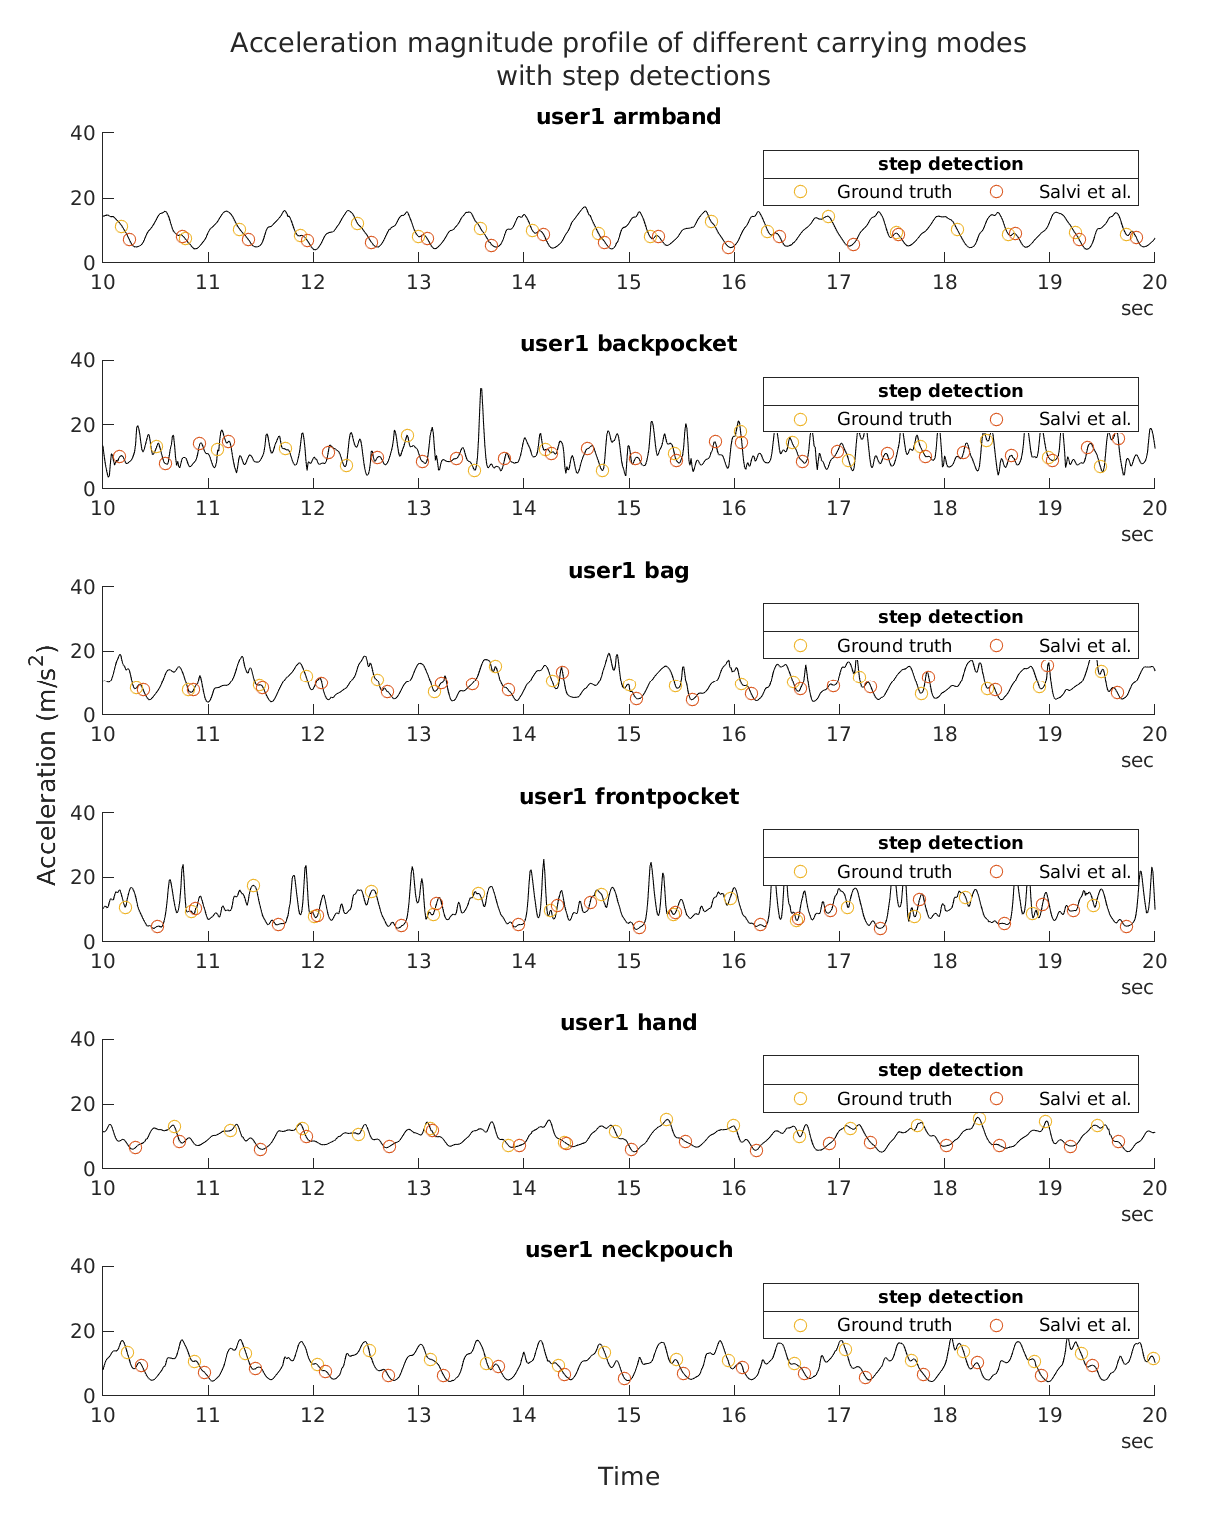
\includegraphics[width=\linewidth]{images/20201112_1318_gt_steps_vs_salvi_steps_1}
	\caption[Step detection validation data]{Extract of validation dataset from \citet{Salvi2018}, indicating ground truth steps and step detected by their algorithm.}
	\label{fig:gt_steps_vs_salvi_steps}
\end{figure}


The step detection method outlined in Algorithm \ref{algo:step_detect} was applied to the validation data of the researchers, allowing for direct comparison. The parameters used for the process coincide with those found by the researchers, an overview of which can be found in \cref{tab:parameters_used}.

\begin{table}
	\centering
	\footnotesize
\begin{tabular}{clc} 
	\hline
	Stage & Parameters & Value \\
	\hline & Window size & $\mathrm{M}=13$ \\
	Filtering & Filter type & Gaussian \\
	& Filter SD & 0.35 \\
	\multirow{2}{*} { Scoring } & & \\
	& Type & Mean Difference \\
	& Window size & $N=35$ \\
	Detection & Threshold & 1.2 \\
	Post-Processing & $t_{\text {window}}$ & $200 \mathrm{ms}$ \\
	\hline
\end{tabular}
\caption{Parameters used in \cref{algo:step_detect}}
\label{tab:parameters_used}
\end{table}

 \cref{fig:sd_abs_comparison} indicates the absolute number of steps detected. \cref{fig:sd_percent_comparison}  shows the percentage error compared to the ground truth, where positive percent error indicates over counting, while negative under counting. The results indicate that the method devised performs overall similarly to the method of the researchers. In some cases the error is slightly larger, as with "user1 bag", while in others it is smaller as with "user 2 bag". It is also apparent that with the case of user1 backpocket that there is a large percentage error for both approaches. The researchers attribute this to the pocket being loose and allowing the phone to rebound when a step was taken \cite{Salvi2018}. This would introduce nefarious components in the accelerometer signal, leading to false positives. \citet{Brajdic2013} encountered similar problems with this carrying position, hypothesizing that the relaxing of the gluteus maximus during locomotion could influence the acceleration trace.
 
	\begin{figure}[htbp]
		\centering
		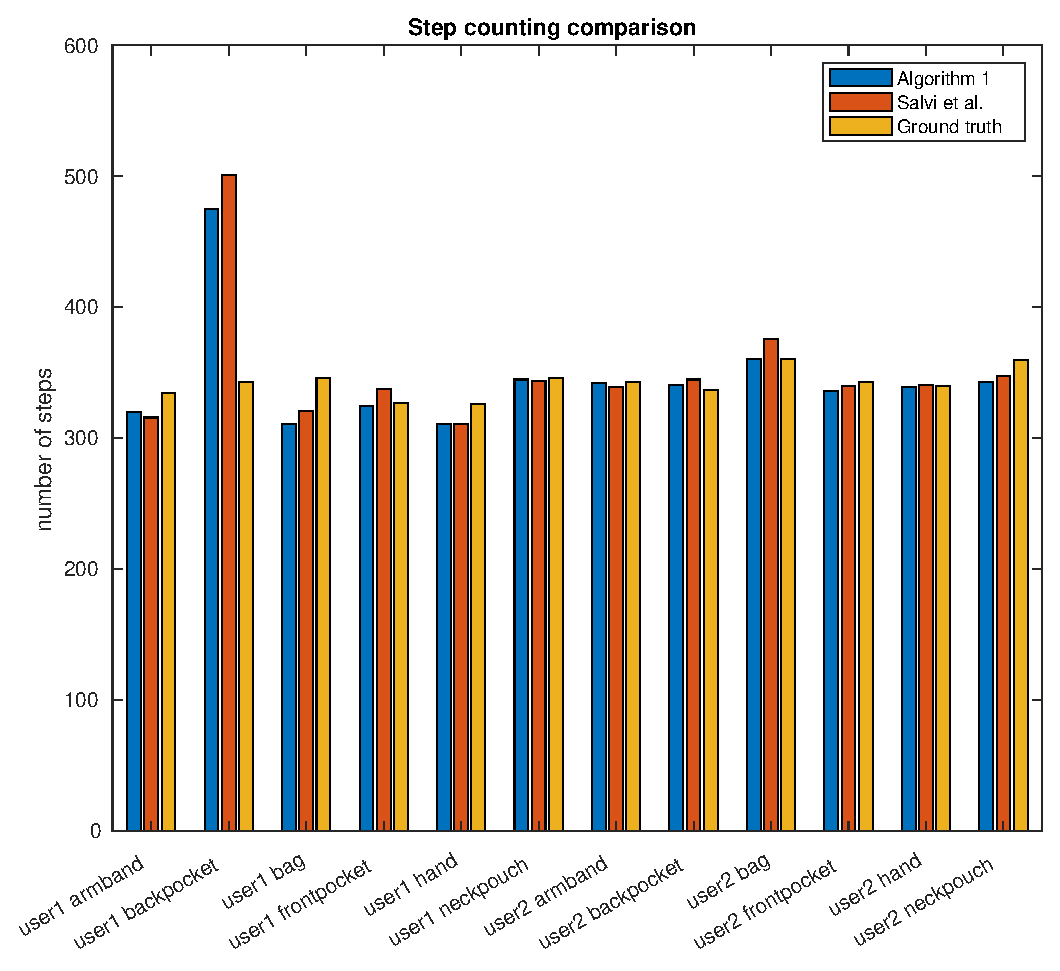
\includegraphics[width=0.7\linewidth]{images/20201112_1347_step_counting_comparison_1}
		\setlength{\belowcaptionskip}{-20pt}
		\caption{Absolute number of steps counted.}
		\label{fig:sd_abs_comparison}
	\end{figure}
\restoregeometry

	\begin{figure}[H]
		\centering
		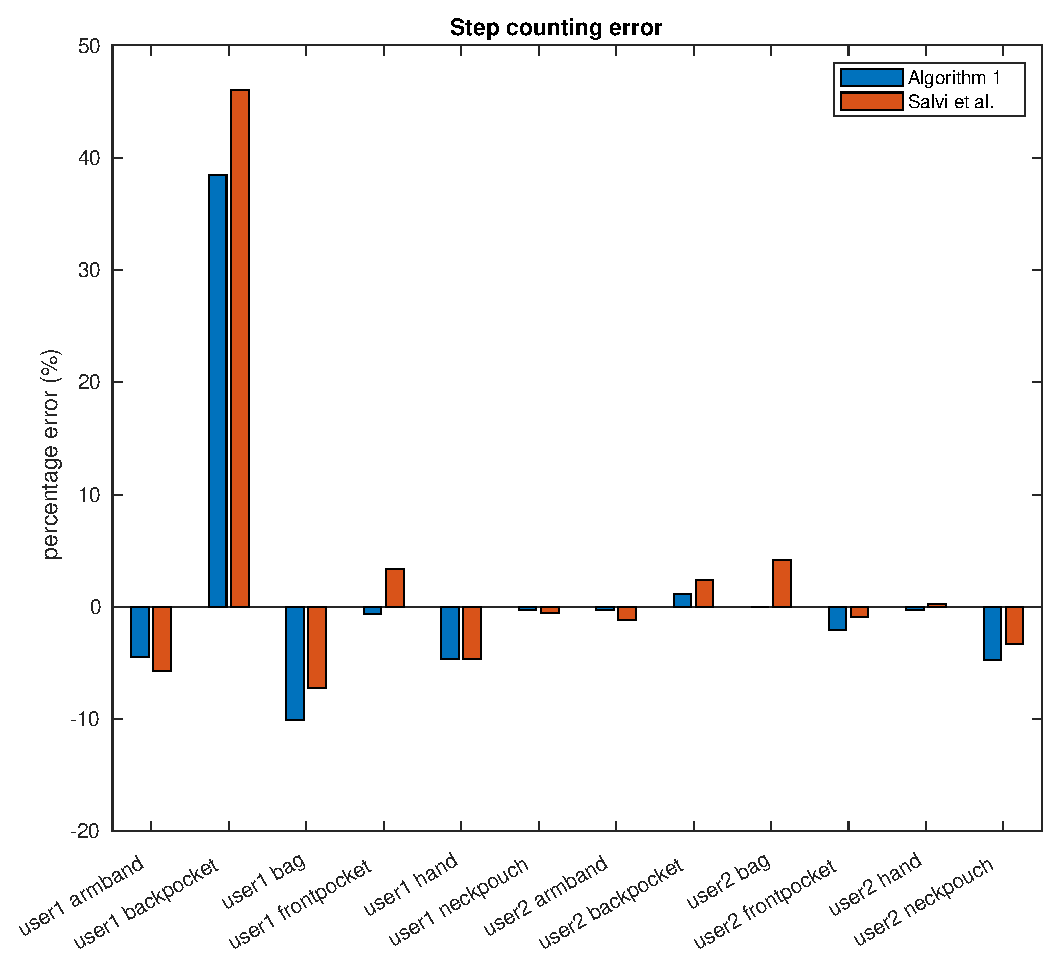
\includegraphics[width=0.7\linewidth]{images/20201112_1401_Step_counting_error}
		\caption{Percentage error from ground truth number of steps. }
		\setlength{\belowcaptionskip}{-2cm}
		\label{fig:sd_percent_comparison}
	\end{figure}
%	\caption[Step detection comparison]{Comparison between \citet{Salvi2018} step detection algorithm, \cref{algo:step_detect} and ground truth for different carrying modes.}
%	\label{fig:sd_comparison}
In addition to the data made available online, original data was gathered outdoors in which I walked exactly 60 steps while having a smartphone in 3 different carrying modes, backpocket, frontpocket and in hand. Two trials per carrying mode were performed. The steps were counted manually. The percentage error from the ground truth can be seen in \cref{fig:202009291013step_counting_error_of_60_steps}. Here the backpocket show similar error as with the validation data, further supporting that the method does not work reliably in this carrying position.
\begin{figure}[H]
	\centering
	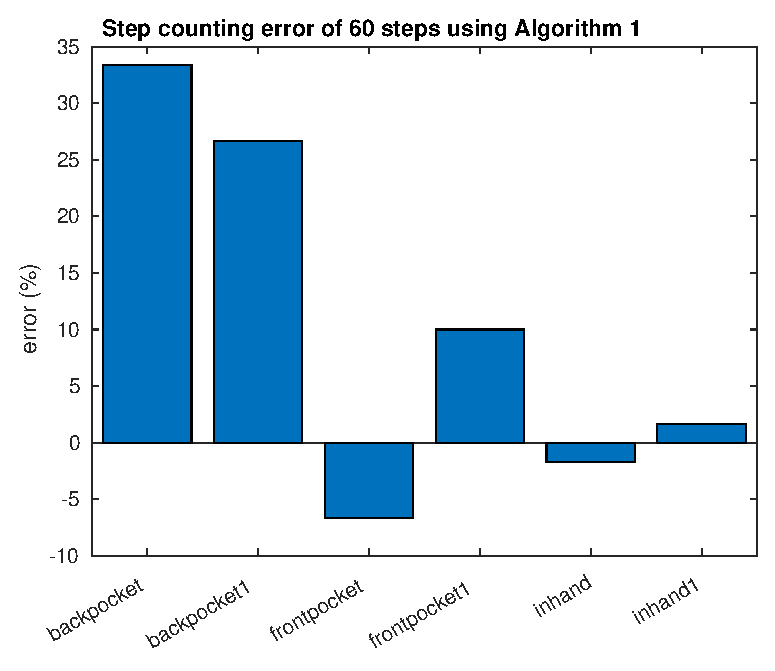
\includegraphics[width=0.58\linewidth]{images/20201112_1406_Step_counting_error_of_60_steps_using_Algorithm_1}
	\setlength{\belowcaptionskip}{-20pt}
	\caption{Original data step counting}
	\label{fig:202009291013step_counting_error_of_60_steps}
\end{figure}

For a PDR SHS it is not enough for the amount of steps to be accurate, but also the time when a step actually occurs. Detecting a step, combined with the heading orientation at that moment, determines the vector in which the position estimate of the pedestrian will move. It is therefore preferable for a detection to be as close as possible to when a step actual occurs, with no other detections close to it. \par
Using the online data, the time difference between a step detection and its closest ground truth point was calculate per trial. The mean and standard deviation of the time difference was calculated, shown in \cref{fig:202011130914smallest_diff_to_gt_1}. Looking at the results this metric indicates that there is no real performance difference between the two approaches as in sometimes one is better than the other and vice versa. The large standard deviations for user2 armband is caused by both step detection methods having already counted multiple steps before the ground truth device has registered any.

\begin{figure}[H]
	\centering
	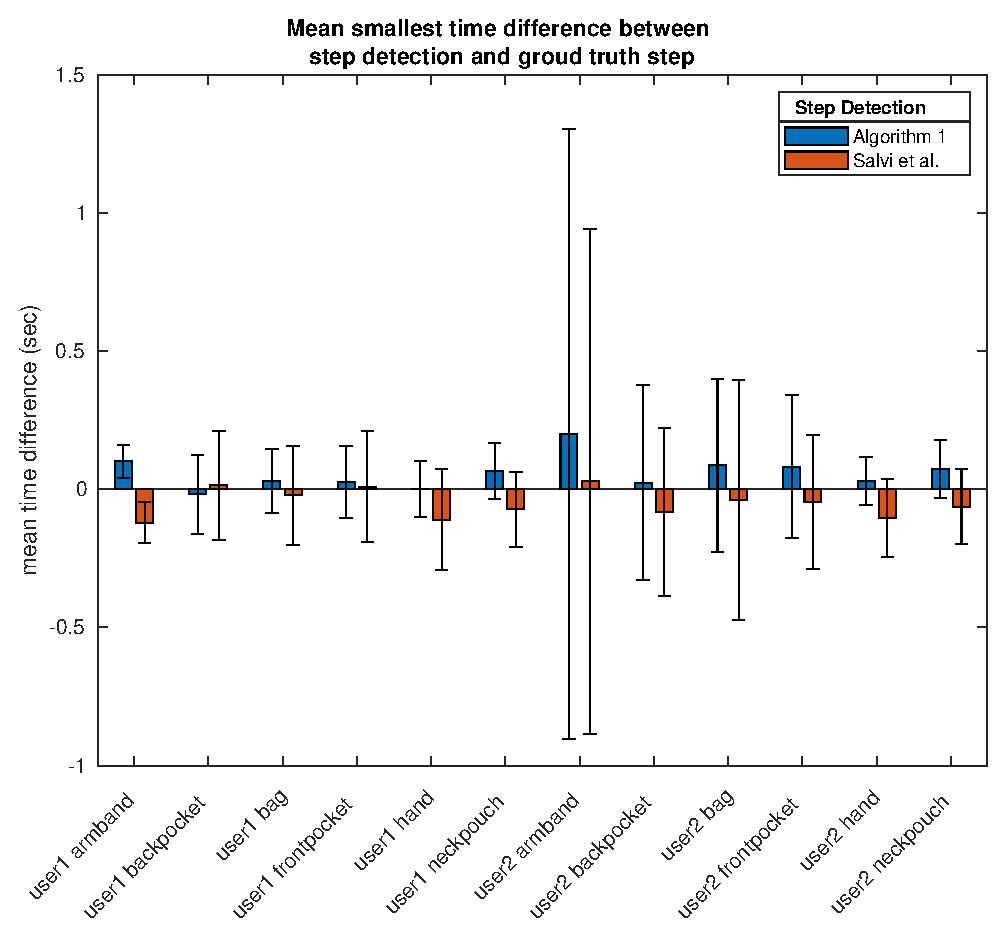
\includegraphics[width=0.7\linewidth]{images/20201113_0914_smallest_diff_to_gt_1}
	\caption{mean smallest time different between step detection}
	\label{fig:202011130914smallest_diff_to_gt_1}
\end{figure}

One problem with this metric is that two subsequent detections may have the same ground truth point as closest point, indicating that there is no unique indication of the step occurring. In order to ascertain how both the \citet{Salvi2018} algorithm and \cref{algo:step_detect} in this respect, an approach to unique step detection was determined. Since it is unrealistic to expect the step detection to be at the exact time an actual step occurs, intervals are defined where if both an actual step occurs and is detected within the interval, the detection counts as a unique step. An illustrative representation of this can be found in \cref{fig:202011121558_true_positive_example_1}. Here an interval, represented by the green region in the graph is made around one of the ground truth points, visible in the middle of the region and circled in red. If in this interval two steps are detected, no unique step is indicated. In the example of  \cref{fig:202011121558_true_positive_example_1},  \cref{algo:step_detect} would be considered a unique step, while the \citet{Salvi2018} algorithm would not, since there are two detection within the interval.

\begin{figure}
	\centering
	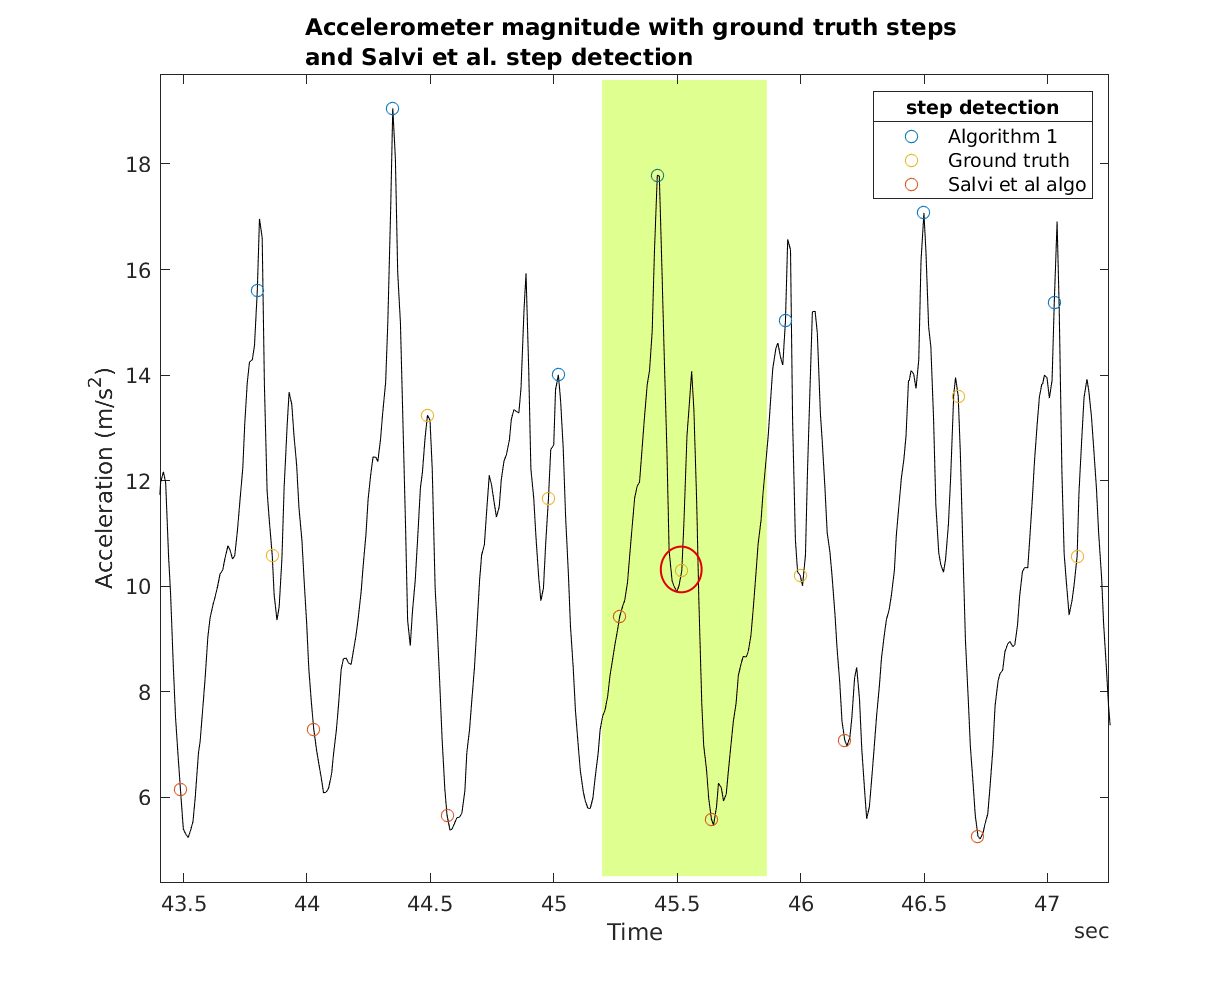
\includegraphics[width=0.75\linewidth]{images/20201112_1809_true_positive_example_2}
	\caption{Representation of interval search method. The light green region represents the search interval around the \citet{Salvi2018} point in the middle.}
	\label{fig:202011121558_true_positive_example_1}
\end{figure}

The time interval is increase itteratively in an attempt to find the highest unique step counts for both algorithms. The results for each user and carrying mode can be found in \cref{fig:sd_tp_fp_comparison}. The results show that while the total number of steps detected are similar between the two approaches, Algorithm \ref{algo:step_detect} has a higher "unique" step detection. This discrepancy between approaches can potentially be explained by the android implementation of the researchers. 

\begin{figure}[H]
	\centering
	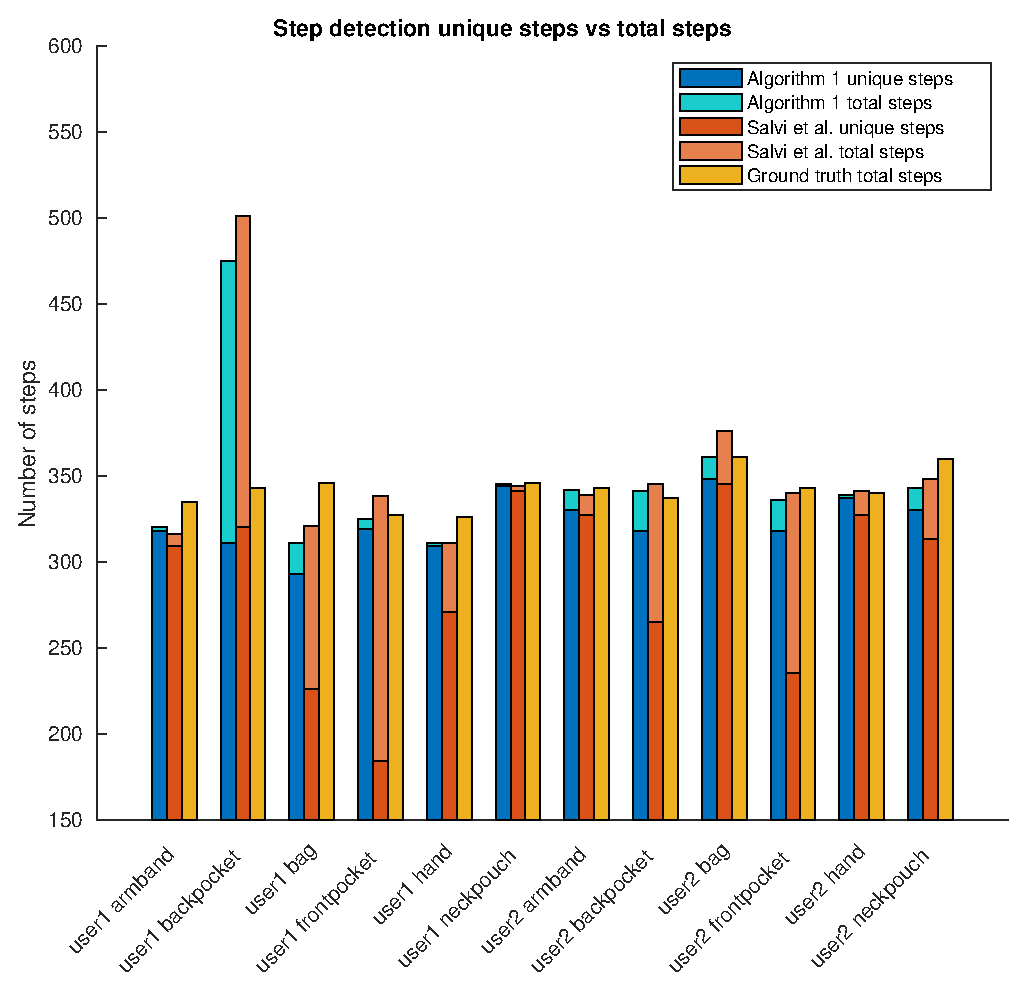
\includegraphics[width=0.7\linewidth]{images/20201112_1857_Step_detection_unique_steps_vs_total_steps_}
	\setlength{\belowcaptionskip}{-20pt}
\caption[False positives and true positives step detection comparison]{Comparison between false positives and true positives for \citet{Salvi2018} step detection and Algorithm \ref{algo:step_detect}}
\label{fig:sd_tp_fp_comparison}
\end{figure}

\section{Step Length Estimation}

\citet{Vezocnik2019} have also made their data available under an open license. This data consists of accelerometer data of 15 different people for three walking speeds and in four smartphone carrying modes. Metrics for each test subject are collected, including height, gender and leg length. The walking speed were qualitative, in that they were either slow, normal, or fast. The carrying modes include the smartphone in a front pocket, in a bag, in the hand with the phone screen parallel to the floor, and in hand will swinging the carrying arm. Each person has two measurements for each combination, one for a 15 meter long straight path and another for 108 meter long straight path. The smaller set is used to determine parameters, while the longer is used to determine performance with the generated parameters. This same process is used in this thesis.\\
The best performing algorithm for global parameters is reiterated in \eqref{eq:Tian2016_sle2} for convenience, where $h$ is the users height and $F$ is the step frequency. The best algorithm for individual parameters is reiterated in  \eqref{eq:weinberg_stepsize2}, where $A_{max}$ and $A_{min}$ are the maximum and minimum acceleration within a step interval. Both approaches will be used and compared to see if similar results are achieved as within \cite{Vezocnik2019}.

\begin{equation}
\label{eq:Tian2016_sle2}
\text{step size} = K \cdot h \cdot \sqrt{F}.
\end{equation}

\begin{equation}
	\text{step size} =K \sqrt[4]{A_{\max }-A_{\min }}.
	\label{eq:weinberg_stepsize2}
\end{equation}

In order to determine the tunable parameter $K$ correctly for both approaches, it needs to be used with the output of the step detection algorithm. This is because step detection will have a direct effect on the step frequency. The step detection algorithm cannot guarantee that all steps are counted, potentially affecting the tunable parameter. 
From the results of step detection, the most accurate results came from holding a smartphone in the hand. This carrying mode is present in the data from \cite{Vezocnik2019}, and will therefore be used for further analysis. \par

The results are shown in \cref{fig:step_length_tian,fig:step_length_weinberg}. Each test subject is shown as a different color with the form of the different markers indicating the speed at which that trial was walked at. In \cref{fig:step_length_tian}, the parameters for \eqref{eq:Tian2016_sle2} of all three walking speeds are plotted. In order to find $K$ as a universal constant, a least square estimation is performed The result is shown by the green striped line in the plot. \cref{fig:step_length_weinberg} shows the same, with the difference being that the parameter is calculate per test subject, instead of all together. 

	\begin{figure}[H]
	\centering
	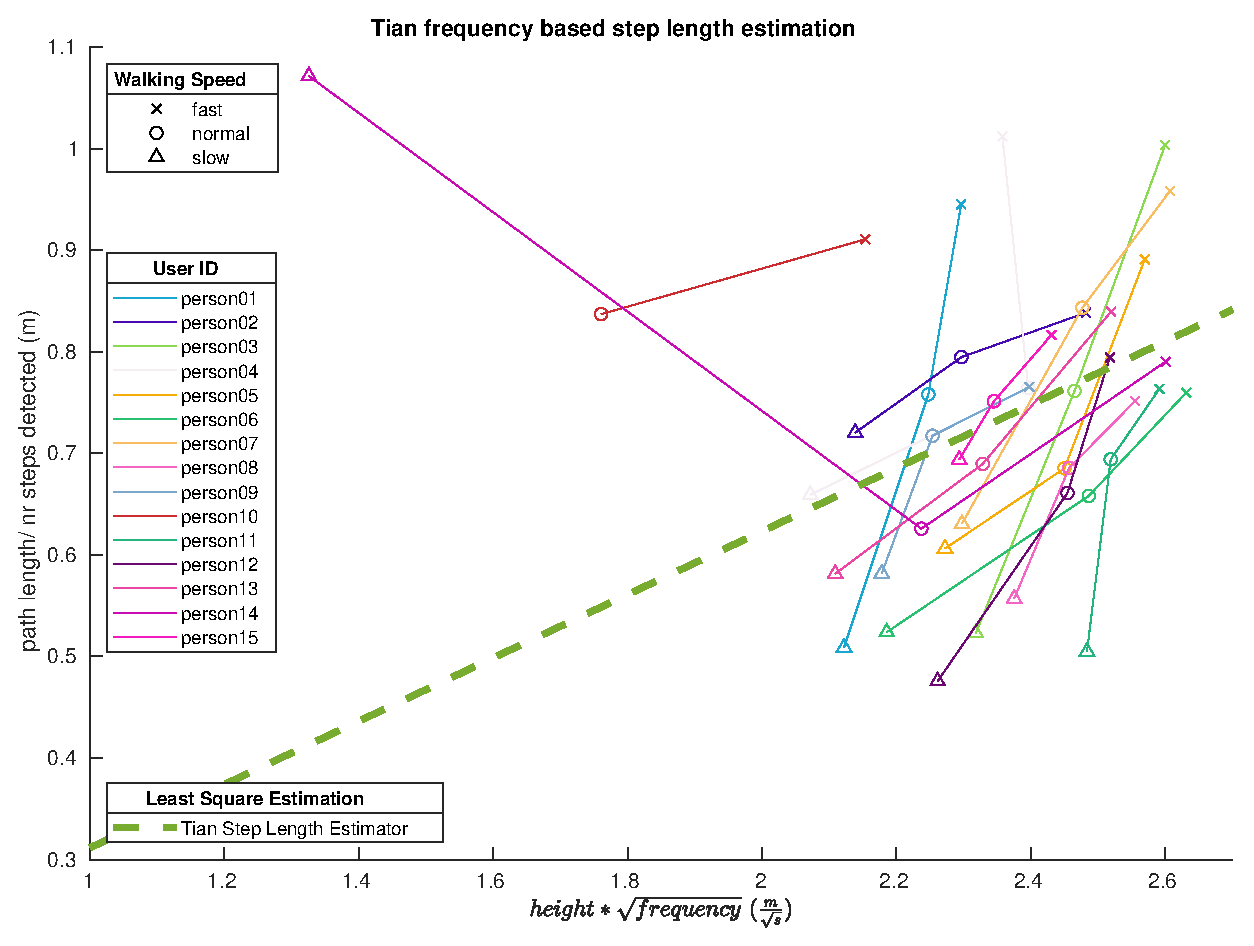
\includegraphics[width=0.8\linewidth]{images/20201113_1634_tian}
	\caption{step length estimation constant = 0.3116}
	\label{fig:step_length_tian}
	\end{figure}
	\begin{figure}[]
		\centering
		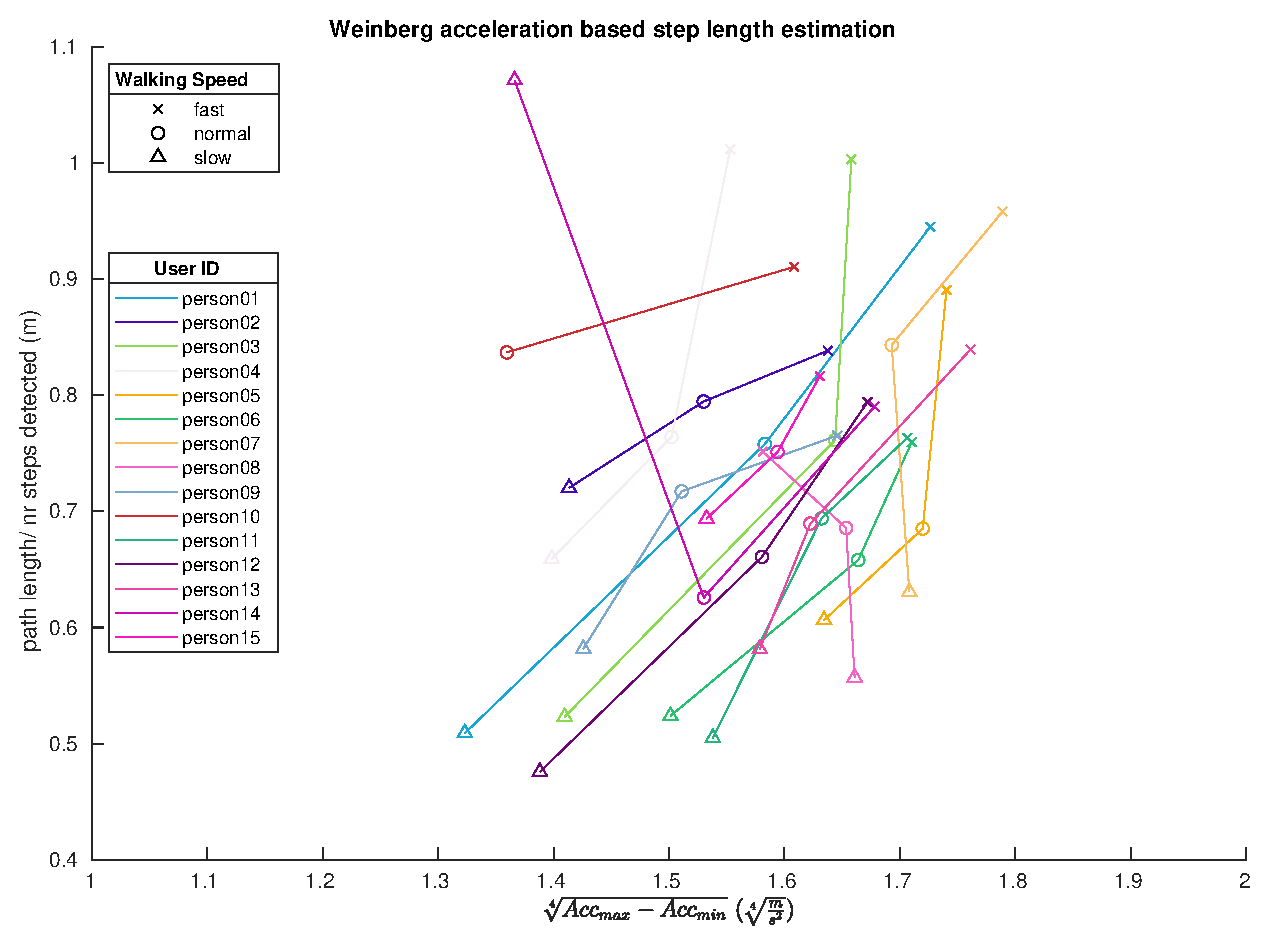
\includegraphics[width=0.8\linewidth]{images/20201113_1639_weinberg}
		\caption{step length estimation constant = 0.3080}
		\label{fig:step_length_weinberg}
	\end{figure}

Using the open source data has not come without problems. While most data seems to follow the general linear relationship, there are two samples that do not. The two potentially faulty data points are the slow walking sample of both person 10 and 14. For the former, no steps have been detected and is therefore not visible in the plots, while for the latter too little steps have been detected. For person 14, 14 steps have been detected for slow walking, which is less steps than when the subject was walking fast. This is either a wrong step detection occurring, or the user walks slowly with very large steps. It is difficult to determine why this is occurring. It could be that during this sample, the test subject was holding the phone incorrectly, the person had a very different step strategy when performing at this speed, or the phone was malfunctioning. This outlier affects the eventual tunable parameter. Removing it will change the estimate from 0.3116 to 0.3080. \par 

The validation dataset can be used to determine if the difference in tunable parameter has a significant affect on the estimate. The results are found in  \cref{fig:step_length_estimation_validation}, where the absolute distance error for all walking speeds for all test subjects are shown, indicated by the dataset ID.
\begin{figure}[H]
	\centering
	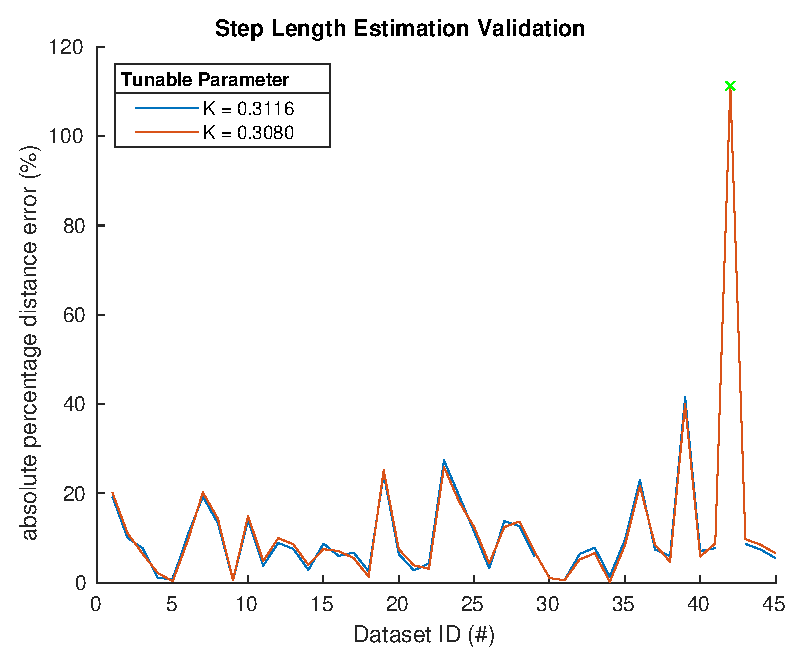
\includegraphics[width=0.7\linewidth]{images/20201028_1344_Step_Length_Estimation_Validation}
	\setlength{\belowcaptionskip}{-20pt}
	\caption{Step length estimation using validation dataset}
	\label{fig:step_length_estimation_validation}
\end{figure}

What is noticeable from the results is that there is a large outlier. This is with dataset 42, which corresponds to the slow walking speed of test subject 14, which is also the setting in which the tunable parameter estimation had an outlier. This further supports that there is something significantly different when this test subject is performing at this walking speed. With this outlier the mean absolute error is 11.8 percent with a standard deviation of 17.1 percent. Without the outlier, the mean absolute error is 9.7 percent with a standard deviation of 8.0 percent. Both results are worse than those cited by \cite{Vezocnik2019}, which indicate a mean of 7 percent with a standard deviation of 5 percent.
The results also indicate that the different tunable parameters do not make a significant difference in accuracy. The difference in performance is likely to the difference in step detection, which the research do specify exactly. \par

The performance of the both step length estimator, applied to the validation set is shown in  \cref{fig:202011131943_wienberg_vs_tian_vezocnik_data1}. This data surprisingly shows that depending on the test subject one or the other method is better at estimating distance traveled. This does not coincide with the results of \cite{Vezocnik2019}, where personal parameters performed better than general parameters.

\begin{figure}[H]
	\centering
	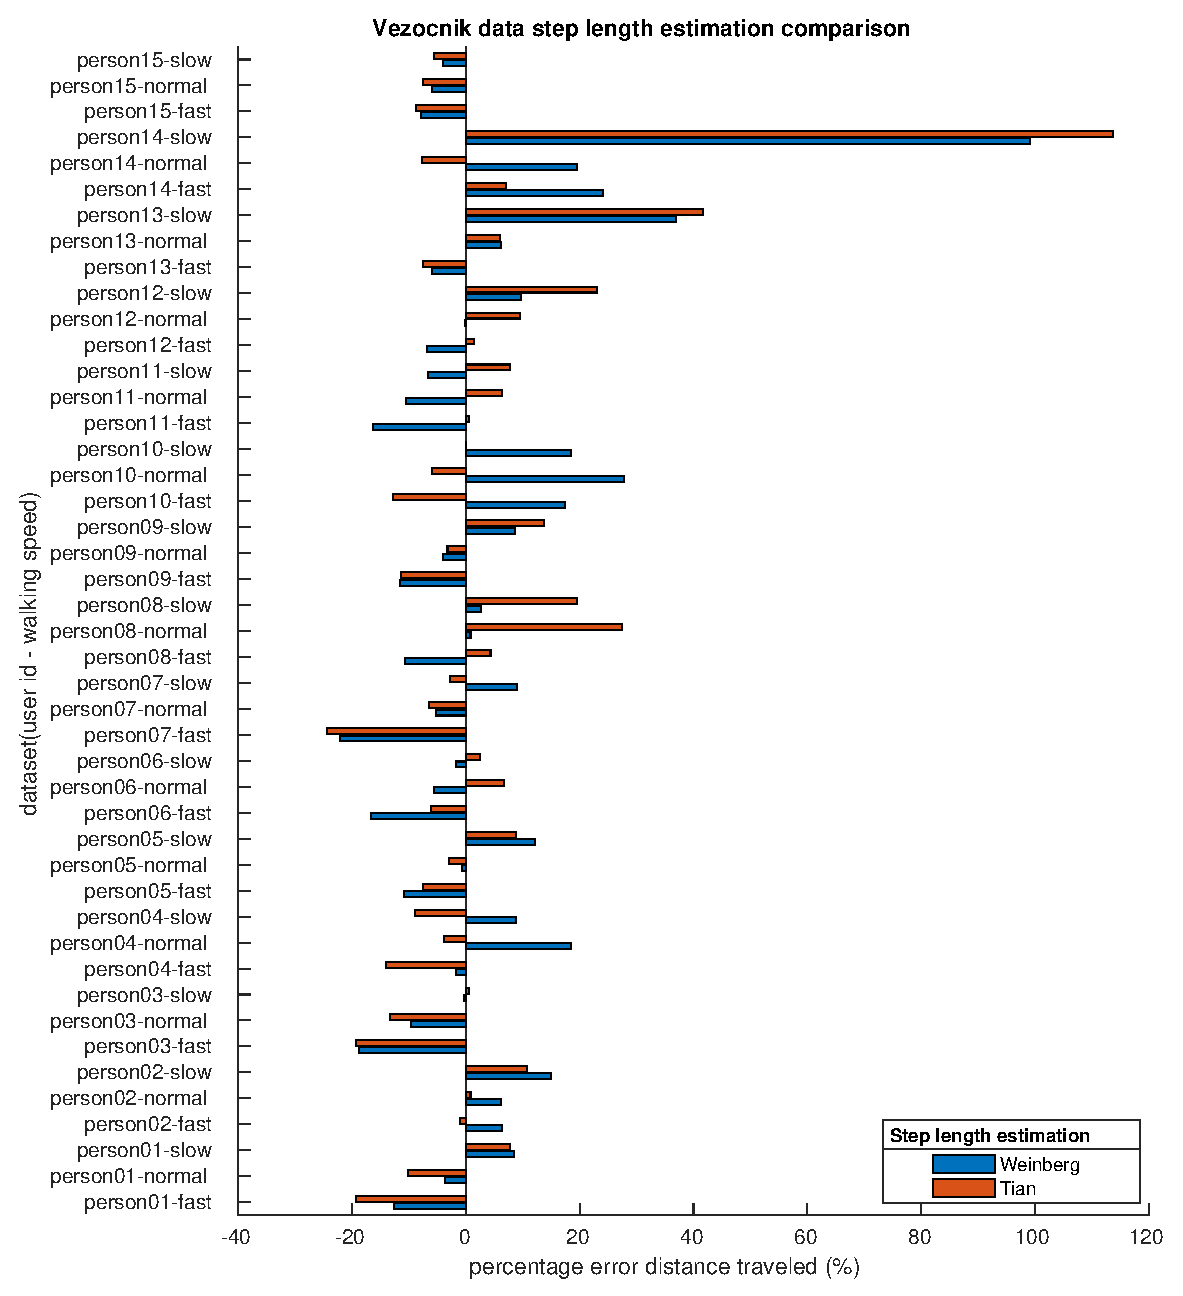
\includegraphics[width=\linewidth]{images/20201113_1943_wienberg_vs_tian_vezocnik_data_1}
	\caption{}
	\label{fig:202011131943_wienberg_vs_tian_vezocnik_data1}
\end{figure}
 
A small scale experiment was performed outdoors where the same process as in \cite{Vezocnik2019} was used. Original data was collected from the same person and device used in the eventual indoor localization experiment. Three trials of 30 meters were walked at different qualitative walking speeds, slow, normal and fast, while recording accelerometer data. Three longer trials of 300 meters were walked, to determine performance. The \citet{Tian2016} method used the same parameter determined for the online data. The \citet{Weinberg2002} parameter was based on the smaller distance data. The results are shown in \cref{fig:step_length_personal_testing}. The results seem to suggest that for slow to normal walking the \citet{Tian2016} method works best, while from normal to fast walking \citet{Weinberg2002} works better. 
\begin{figure}[H]
	\centering
	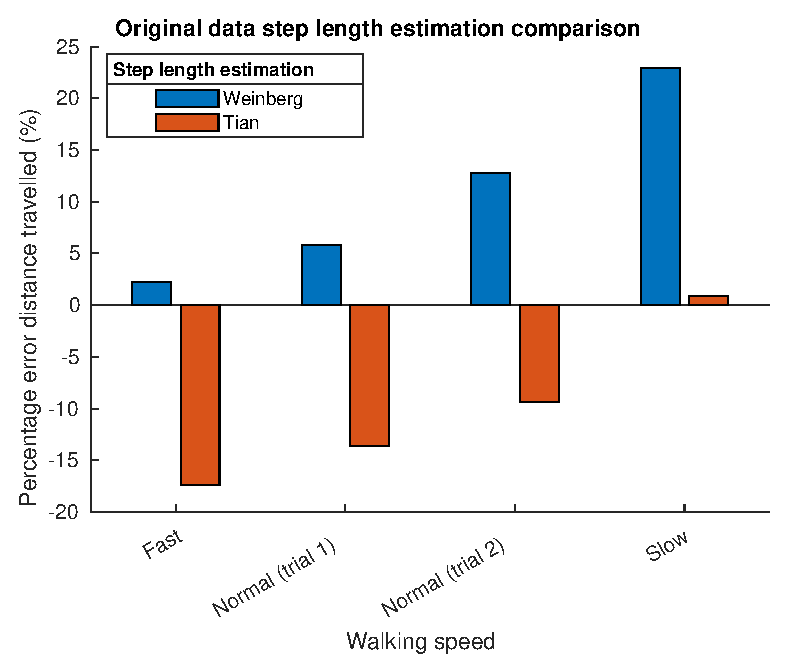
\includegraphics[width=0.7\textwidth]{images/20201113_1920_wienberg_vs_tian_og_data_1}
	\caption{Original data step length estimation \\ }
	\label{fig:step_length_personal_testing}
\end{figure}

{\color{cyan} still need to add comment on results of test with original data and see how it compares with the data from \cite{Vezocnik2019}... The results so far show that general parameters are not good. In the experiments indoor }

\textcolor{red}{I think that step length estimation is one of the largest error sources ATM. Is it work while switching to a different technique? \citet{Vezocnik2019} also indicate on that is good for personalized parameters ....? I think that this could be fixed quickly}

\section{Indoor Orientation Estimation}

The step detection and step length estimation experiments were performed outdoors, since the location has no effect on accelerometer readings and outdoor testing allows for longer walking distances. Orientation estimation and the whole system performance naturally are location dependent, and will have to be tested indoors. \par

Indoor testing was located at the house of a family member. The test consisted of walking around indoors with a smartphone in hand, and recording the IMU signals in the phone through a dedicated android app. Using the smartphone data, the SHS trajectory could be calculated. During the experiment, a total of 6 successful trials were walked by one test subject, each trying to generate a different trajectory than the previous trials. This same test subject was also used for step detection and step length estimation experiments.

\section{Overall System Testing}

During the experiment, a smartwatch was worn around the wrist of the hand that was not holding the smartphone. This hand was used to open and close doors. The opening of doors was also recorded through the app on the smartphone, which had a button to record timestamps when pressed. The full experimental process can be found in \cref{appendix:shs_experiment}. \par

The smartwatch accelerometer data was synchronized with the smartphone data. The activity recognition method in \cref{sec:method-AR} was used to try and detect door interaction. Combining the activity detection and  with the floor map generated in \cref{sec:method-pf}, the whole system could be tested. For initialization a known starting location on the map was indicated, around which the particles were distributed with a Bayesian profile.  \par 

In addition to recording IMU data from both smartphone and watch while the path was being walked, the trials were also being filmed from a breast pocket by another smartphone. The video recorded during the experiment was used to get a rough estimate of the path walked during the trial. This was done by replaying the video and pausing it at one second intervals. At the paused moments, the test subject position was manually indicating on the map The position and time elapsed since the start of the trial were recorded. The resulting trajectory can be used to give some performance indication of the devised method. \par 

\subsection{With "perfect" activity recognition}
During the experiment the possibility existed of recording a timestamp to indicate the beginning of interaction with a door within the indoor environment. This could be used as a ground truth comparison for eventual activity recognition, but also as a way of representing perfect activity recognition. The recorded timestamps can be used as a particle filter measurement update. Using this method the potential affect of activity recognition for indoor localization can be evaluated, by comparing performance when this form of measurement is used and not used. \par 

All trials were run through the complete system with the manually recorded door interactions, with 3000 particles. This was done for five iterations per trial, in order to show reproducibility.  The resulting estimated trajectory was then compared with the rough estimate generated from video.  A root mean square error was calculated between the two, the results of which can be found in \cref{fig:pf_boxplot}.

\begin{figure}[H]
	\centering
	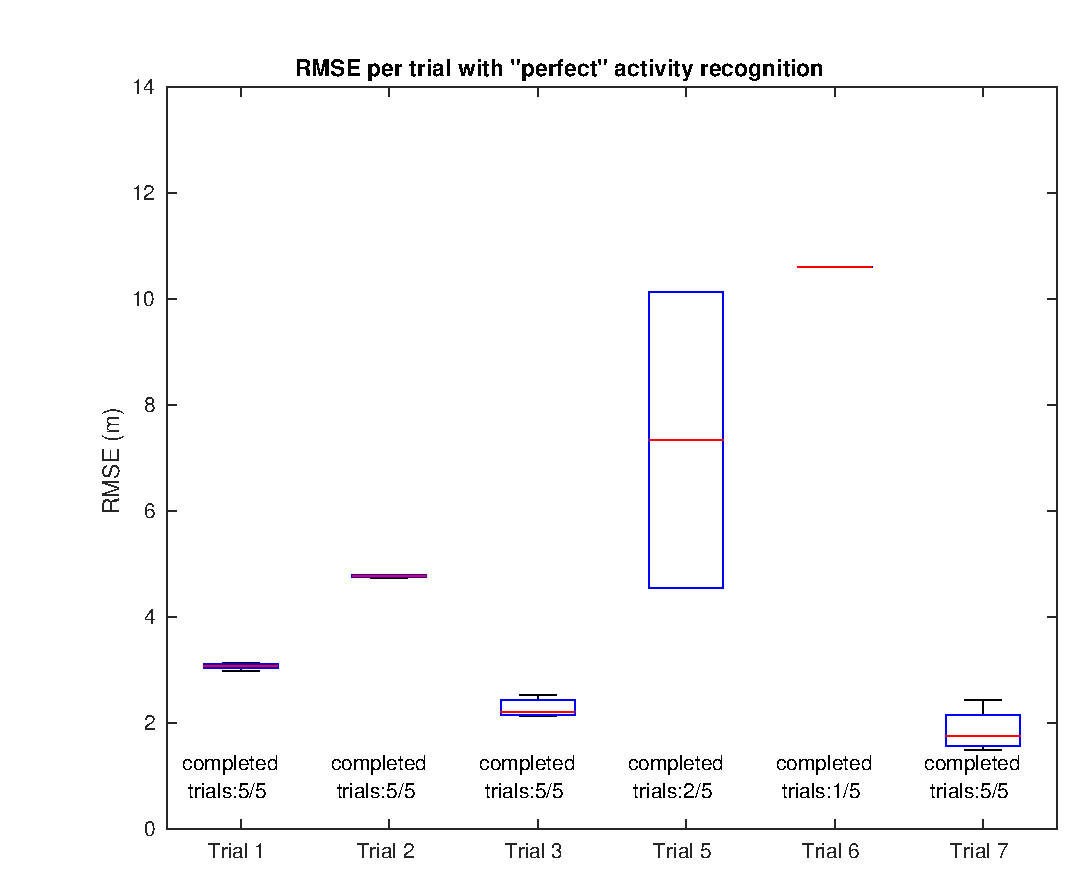
\includegraphics[width=0.6\textwidth]{images/20201116_1332_RMSE_per_trial_with_perfect_activity_recognition}
	\caption[Particle Filter position estimation performance with door interaction]{Particle Filter position estimation performance with rough video generated estimate using manually indicated door interactions}	
	\label{fig:pf_boxplot}
\end{figure}

The results show that for trials 1 to 3 and trial 7 that all five itterations were completed, with their individual itterations have similar RMSE values. The RMSE per trial do vary, which can be explained by looking at the trajectory that the system generates. \par 

\begin{figure}[H]
	\centering
	\begin{subfigure}[t]{.45\textwidth}
		\centering
		\begin{tikzpicture}
			\node[anchor=south west,inner sep=0] (image) at (0,0) {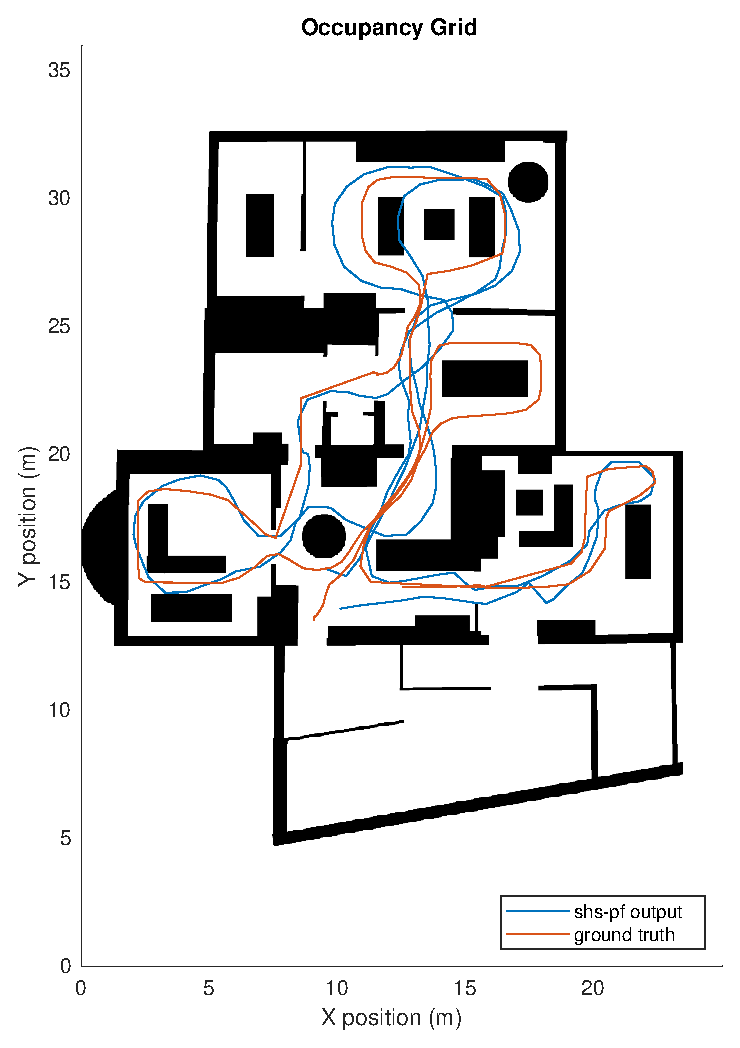
\includegraphics[width=0.9\textwidth]{images/20201029_1603_shs-pf_trial_1_2}};
			\begin{scope}[x={(image.south east)},y={(image.north west)}]
				\draw[green,ultra thick,rounded corners] (0.6,0.625) rectangle (0.73,0.66);
			\end{scope}
		\end{tikzpicture}		
		\caption{trajectory comparison}
		\label{fig:shspf_trial1_on_map}
	\end{subfigure}
	\begin{subfigure}[t]{.45\textwidth}
		\centering
		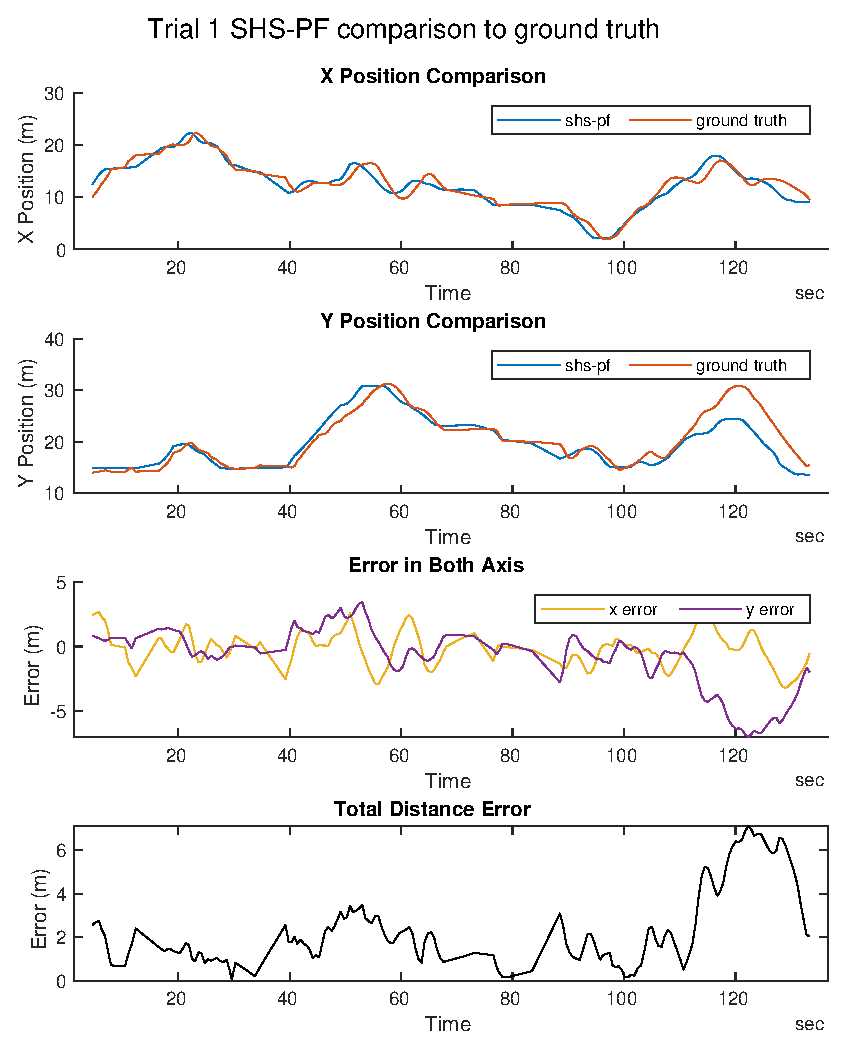
\includegraphics[width=\linewidth]{images/20201029_1603_shs-pf_trial_1_1}
		\caption{axis comparison}
		\label{fig:shspf_trial1_comparison}
	\end{subfigure}
	\setlength{\belowcaptionskip}{-20pt}
	\caption{SHS-PF comparison of trial 1 with ground truth}
	\label{fig:shspf_trial1_shs_gt_comparison}
\end{figure}




\subsubsection{Without activity}
The same SHS trajectory were used, however now door interaction landmarks were not used as measurement update. The results can be found in \cref{fig:pf_boxplot_no_doors}.

\begin{figure}[H]
	\centering
	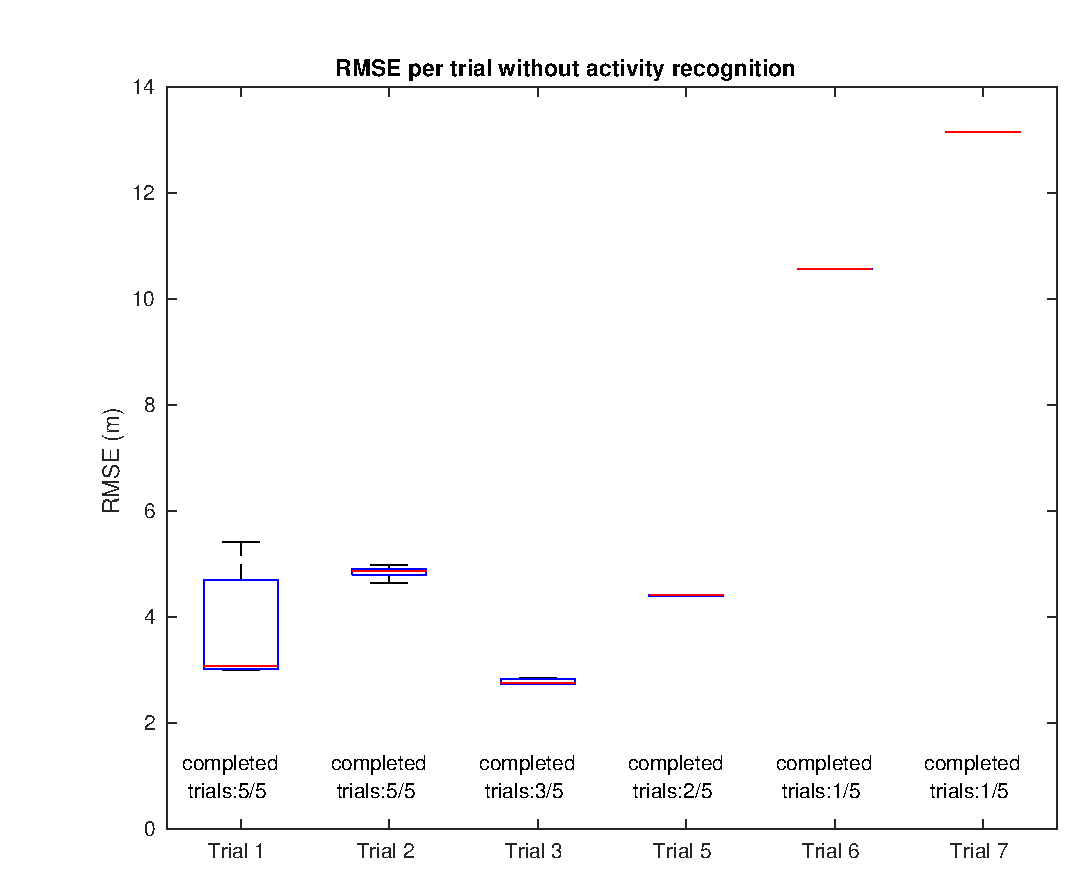
\includegraphics[width=0.7\textwidth]{images/20201116_1333_RMSE_per_trial_without_activity_recognition}
	\caption[Particle Filter position estimation performance without door interaction]{Particle Filter position estimation performance without door interaction measurment update, 5 itterations per trial. Number under "completed" indicates how many trials had particles surviving for the whole SHS trajectory.}
	\label{fig:pf_boxplot_no_doors}
\end{figure}

\textcolor{purple}{
	things to notice
	\begin{itemize}
		\item Trial one has very different RMSE value per run
		\item Strangely it did not have much effect on lopen1.2
		\item Although the RMSE of lopen1.3 is similar to the one with door activity two of the 5 trials did not complete the SHS track. This means that all particles.
		\item So far this does indicate that having activity recognition does help with position estimation within a particle filter
\end{itemize}}


\subsection{Indoor Orientation Estimation}
The indoor orientation estimation method outlined in \cref{sec:method-EKF} can be compared with the output of the android operating system. Two examples can be found in 

\begin{figure}[H]
	\centering
	\begin{subfigure}[t]{.45\textwidth}
	\centering
	\includegraphics[width=0.7\textwidth]{example-image-a}
	\caption{Orientation estimation of trial 1 compared to android orientation estimation}
	\label{fig:trail1 - shs}
\end{subfigure}\quad
\begin{subfigure}[t]{.45\textwidth}
	\centering
	\includegraphics[width=0.7\textwidth]{example-image-b}
	\caption{Orientation estimation of trial 2 compared to android orientation estimation}
	\label{fig:trail2 - shs}
\end{subfigure}
\end{figure}

These two examples indicate that the two estimation techniques have a similar performance. There is no reason for a direct comparison between the orientation estimation outline in \cref{sec:method-EKF} and the attitude estimation of the, since this will be relative to each other and not to the ground truth which is not available. 

A rudimentary comparison could be made using the ground truth of the experiment, where the assumption is made that the angle of the displacement vector can be considered the orientation of the phone. The different orientations can be compared by showing the difference in angle for the initial orientation. An example of this can be found in \cref{fig:orientation_comparison}, also showing the orientation estimations of the phone and the EKF method.

\begin{figure}[H]
	\centering
	\includegraphics[width=0.6\textwidth]{example-image-c}
	\caption{Orientation distilled from ground truth compared to orientation estimation of android system and EKF}
	\label{fig:orientation_comparison}
\end{figure}

The error between each trial and the orientation distilled from the ground truth trajectory can be found in \cref{fig:orientation_error_comparison}.

\begin{figure}[H]
	\centering
	\includegraphics[width=0.6\textwidth]{example-image-c}
	\caption{Error between ground truth orientation and android system and EKF}
	\label{fig:orientation_error_comparison}
\end{figure}


{\color{red}As can be seen this plot has not been generated yet. Depending on the outcome a comparison can be made over all trials to determine performance of the different methods. What do you think, is this a valid way of comparing orientation estimate?}


\subsection{Step Length Estimation}

\textcolor{red}{is it worthwhile to compare step length estimation with the video ground truth generated?}

\subsection{Step and Heading System}

\textcolor{cyan}{trial naming at this point is not consistent, also not in the plots ... needs to be changed}

All components of the step and heading system have been tested separately, giving an indication of their strengths and limitations. Now the whole system can be combined and tested in an indoor environment to evaluate the complete system performance.
For every trial the smartphone IMU data is passed through the different components of the SHS outlined in this report. Each trajectory can then be compared to the ground truth generate through post processing as outlined at the beginning of this section. Two trials with their trajectory projected onto the map and side by side comparison with the ground truth can be found in \cref{fig:trial1_shs_gt_comparison} and \cref{fig:trial2_shs_gt_comparison}. Note that the shs trajectories in these images have been rotated heuristically in order to fit the map as best as possible. This needs to be done since there is no way for the step and heading system output to know how to orient itself with respect to the building. This is because it does not have pre-existing knowledge on the orientation of the magnetic field inside the building. Since this heuristic rotating is only used to give an indication of the shs output compared to the ground truth, it is not possible to compare it quantitatively with the ground truth, since it is not a standalone solution for indoor localization.

\newpage
\subsection{Activity Recognition}
\textcolor{cyan}{
\begin{itemize}
	\item calculate the difference between the ground truth start of door interaction and the begin of the simple decision tree method outlined in the thesis
\end{itemize}}

\textcolor{red}{What do you think is also important to show about activity recognition}

